\chapter{Plataformas}
\label{chap:Plataformas}

Para a localização com os residuos de comunicação \emph{WiFi} são necessários
sensores que possam capturar estes residuos e processar qualquer informação
capturada por esse sensor. Esta plataforma de sensor pode ser construida com
qualquer plataforma computacional capaz de ser programada com comunicação
\emph{WiFi} porém o \emph{hardware} de \emph{WiFi} e seu \emph{software}
controlador deve permitir o Modo Promíscuo.

Este Modo Promíscuo (\emph{promiscuous mode}) é definindo pela capacidade de uma
Placa Adaptadora de Rede \emph{WiFi} (\emph{Network Interface Card} -
\emph{NIC}) receber e interpretar todos os pacotes que trafegam em uma rede ou
em todas as redes que estão em seu alcance, independentemente do destinatário do
pacote. Em seu fucionamento normal uma \emph{NIC} descarta todos os pacotes que
não são destinados para ela o mais cedo possível evitando reprocessamento de
dados indesejáveis, por este motivo não são todas as \emph{NICs} que permitem o
Modo Promíscuo Essa funcionalidade elimina a necessidade de \emph{hardware} ou
\emph{software} em cada um dos dispositivos rasterados.

Neste sentido elegeram duas plataformas de notável importância no mercado atual
e notável facilidade de acesso para qualquer interessado na área. As plataformas
testadas são o microcomputador \emph{Raspberry Pi} e o microcontrolador
\emph{ESP8266}. Ambos  foram escolhidos pelo domínio do segmento de Prototipação
e Faça Você Mesmo  (\emph{Do It Yourself} - \emph{DYI}) dentro do campo de IoT.
Outro líder de segmento, o \emph{Arduino}  foi prontamente descartado por não
conter nativamente a habilidade de conectar-se à \emph{internet} sendo
constantemte combinado com um dos escolhidos para ganhar esta habilidade
demonstrando claramente menor afinidade a este projeto em comparação aos seus
igualmente famosos concorrentes.

Após escolhidas as plataformas de intersse alguns exemplares de cada uma delas
foi adquirido para implementar a aplicação proposta. Neste sentido, serão
apresentadas cada uma dessas plataformas quanto as suas especificações técnicas
e aos produtos utilizados em conjunto para que elas pudessem funcionar e serem
programadas e os motivos pela adoção ou não delas.

\section{ESP8266}

O ESP8266 é um SOC (\emph{System On a Chip} -  Sistema em um \emph{chip}), ou
seja, é um chip com todos os circuitos eletrônicos necessários e partes para um
dado sistema em único cirtuito integrado. Este chip possui:

\begin{alineas}

	\item \emph{WiFi} embutido com capacidade de 2,4 GHz (802.11 b/g/n);

	\item 16 GPIOs (\emph{general-purpose input/output}) - I2U, SPI, UART,
entrada ADC, saída PWM;

	\item Arquitetura RISC de 32 bits para segurança \emph{WiFi};

	\item CPU que opera em  80 MHz, com possibilidade de operar em 160 MHz;;

	\item 64 KB de ROM para \emph{boot};

	\item 64 KB de RAM para instruções;

	\item 96 KB de RAM para dados;

	\item  Memória \emph{Flash SPI} de 512 KB a 4 MB (dependente de módulo externo);

	\item Núcleo baseado no \emph{IP Diamand Standard LX3} da \emph{Tensilica}.

\end{alineas}

Para o mercado de prototipação, fabricantes constroem placas de diferentes
configurações com este chip como elemento central, os chamados módulos. Estes
módulos usam o ESP8266 com diferenças perceptíveis, por exemplo, quantidade de
pinos, dimensões físicas e alguns podem até operar de modo \emph{standalone}
(sem outro \emph{hardware} de suporte como reguladores de tensão, conversores
serial-USB) e especialmente a \emph{Memória Flash SPI}. Neste trabalho, foram
usados os módulos: ESP-01, LoLin, D1 mini e ESP-12F.

\begin{figure}[htb]
	\caption{\label{fig:modulos-esp}Módulos ESP8266 Adquiridos}
	\begin{center}
		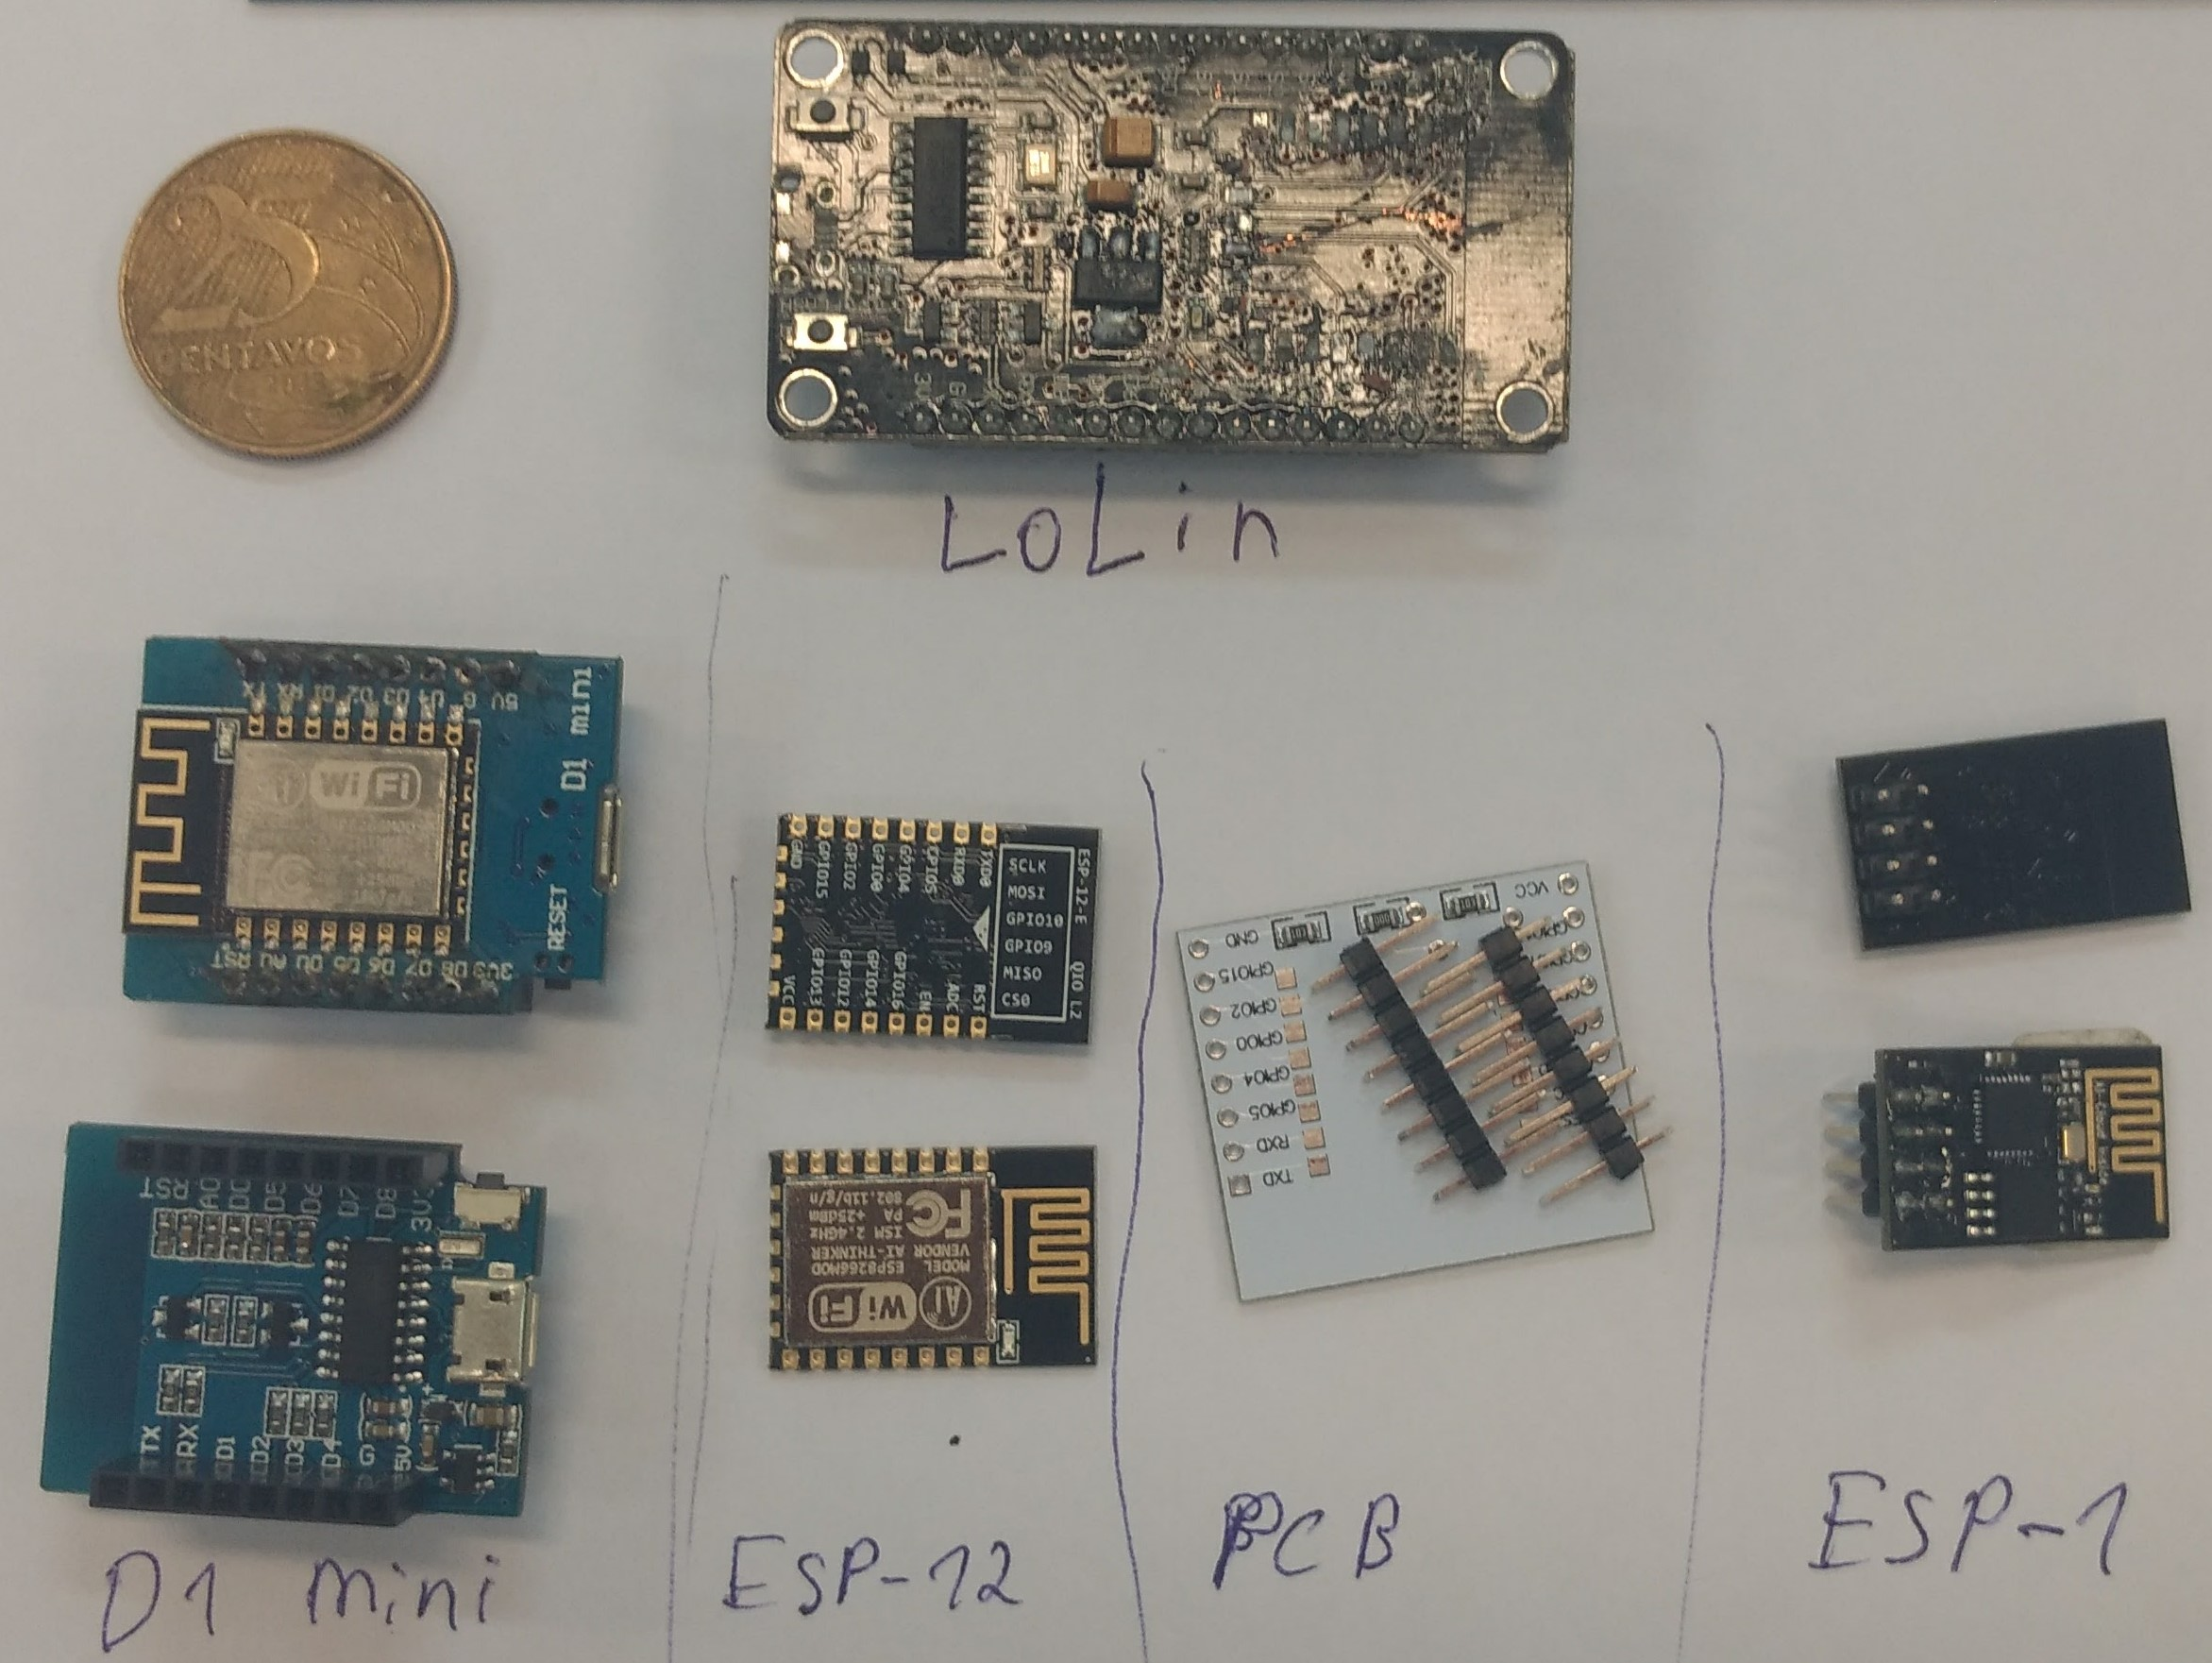
\includegraphics[width=1\textwidth]{040-plataformas/modulos-esp.jpg}
	\end{center}
	\legend{Fonte: Elaborada pelo autor}
\end{figure}

\begin{figure}[htb]
	\caption{\label{fig:modulos-esp}Programação de um módulo ESP-12f com \emph{breadboard}}
	\begin{center}
		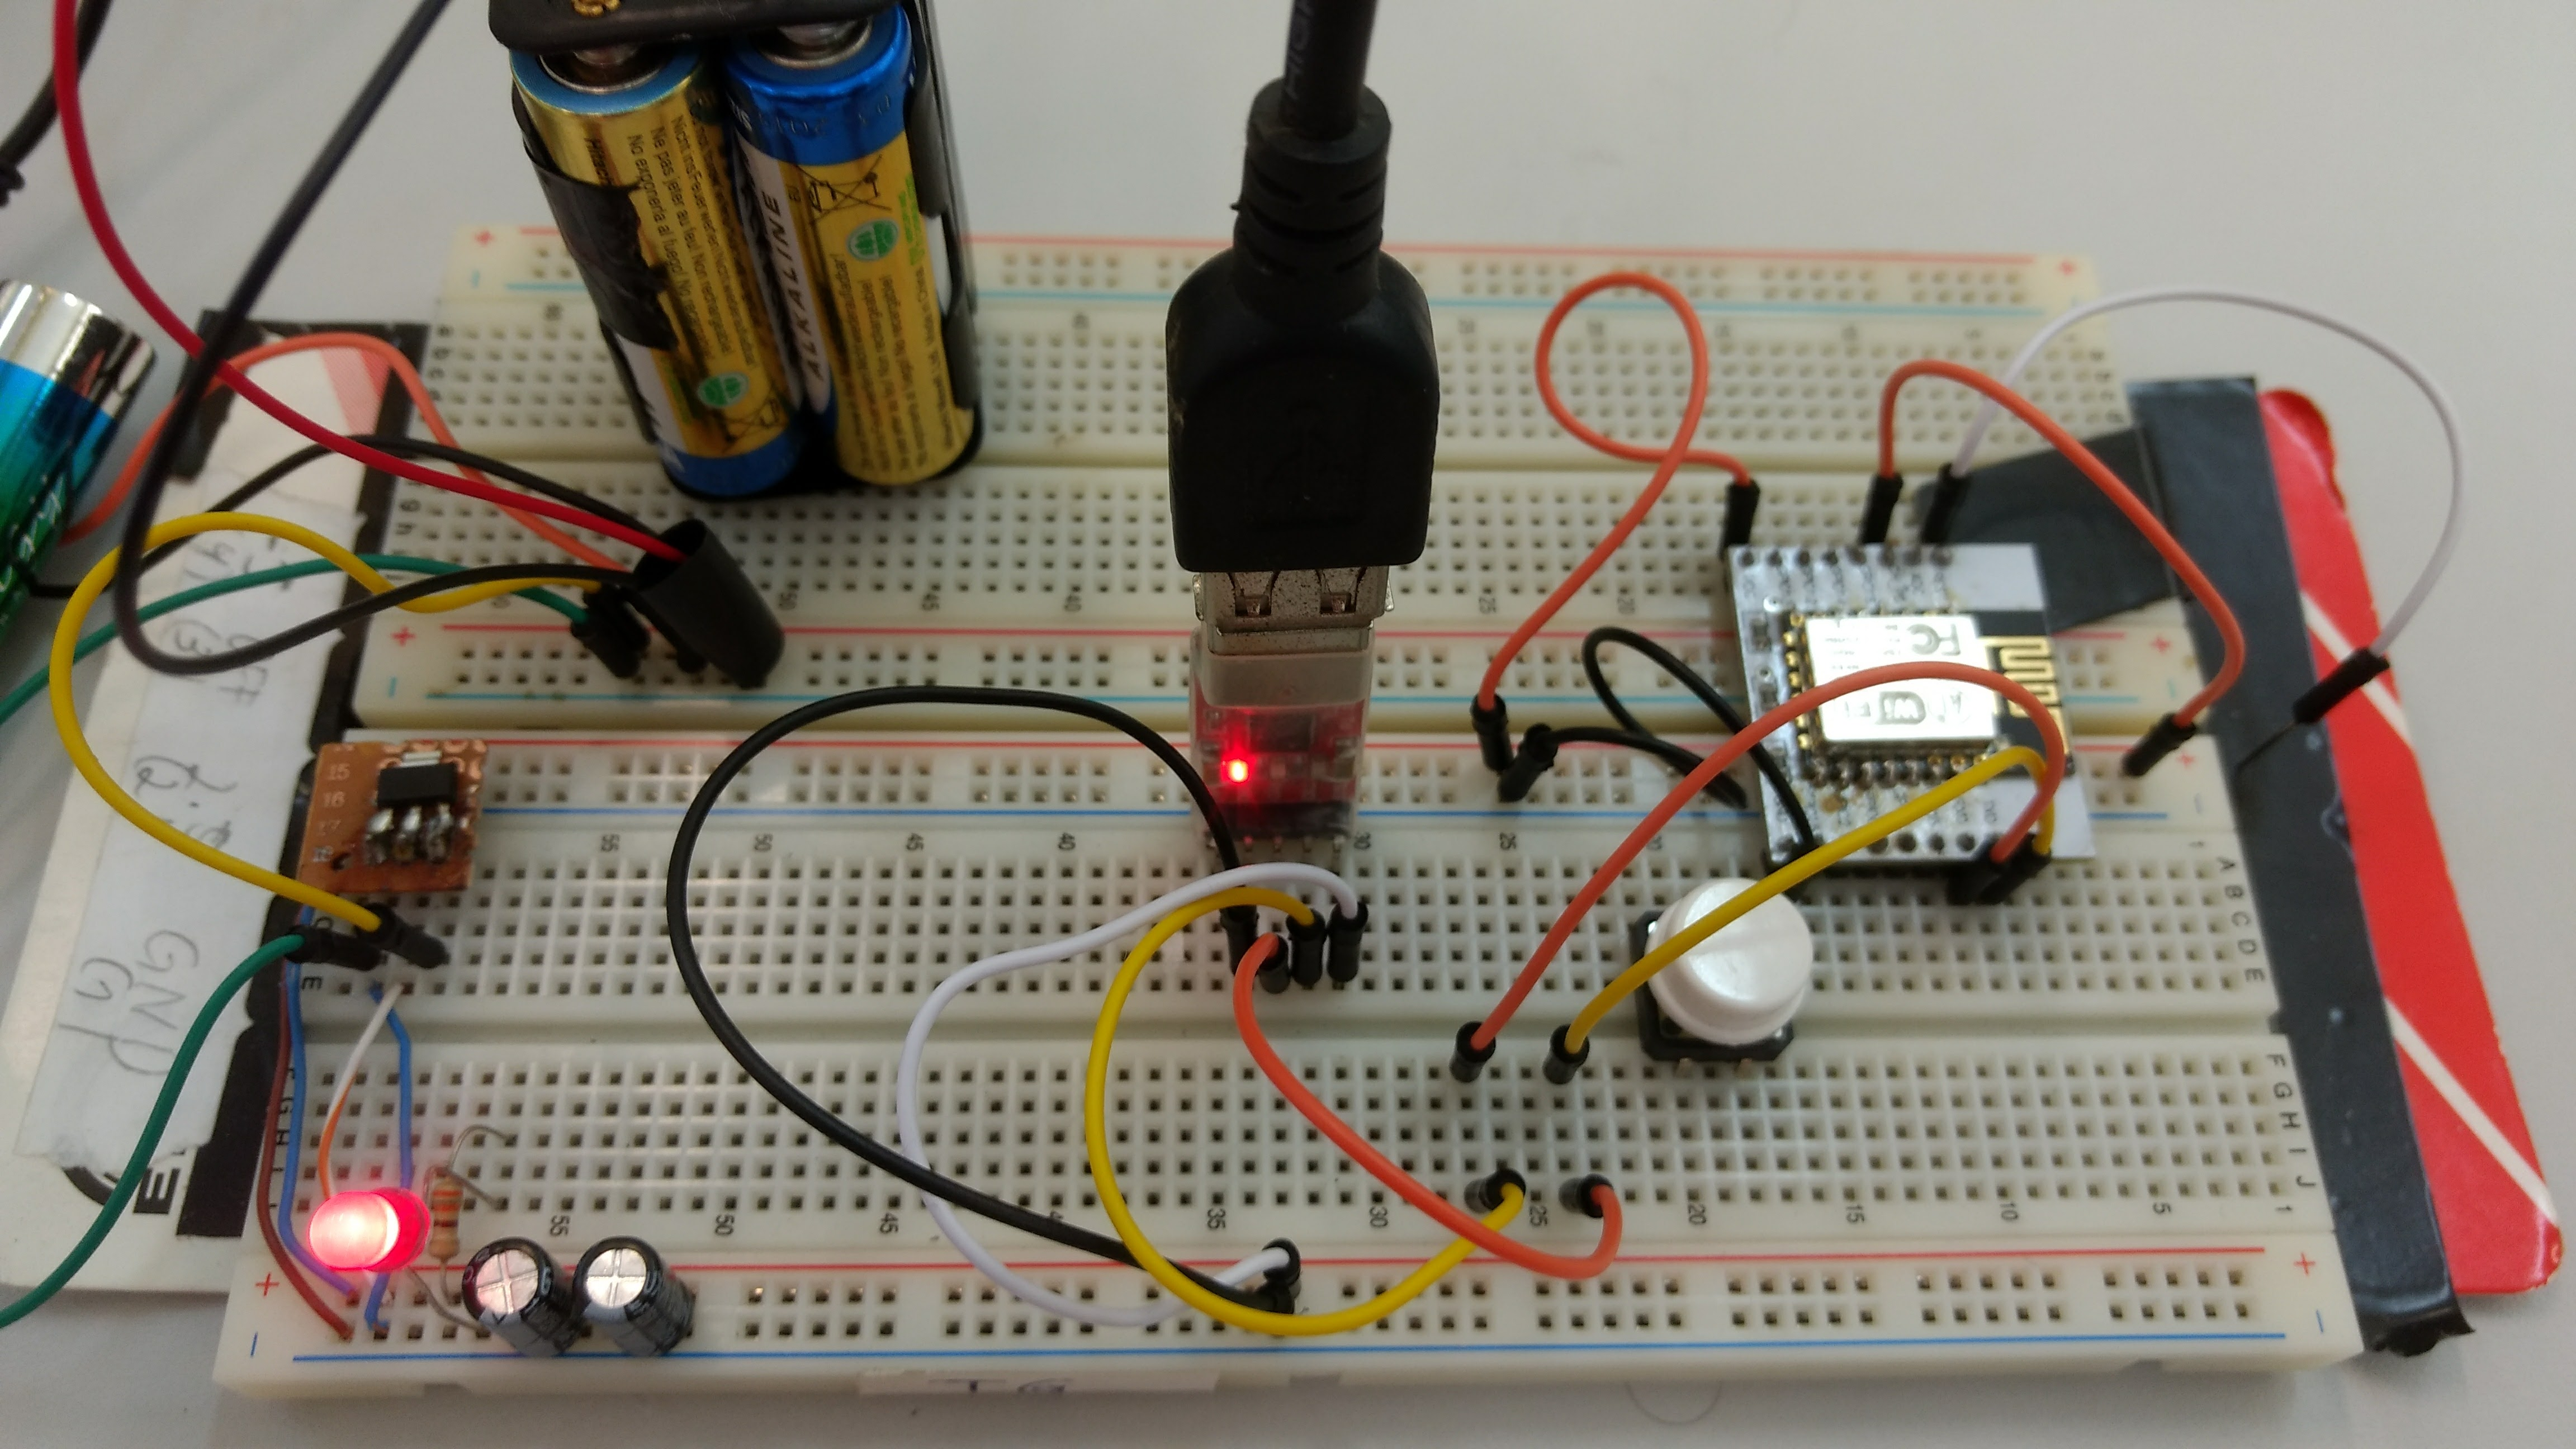
\includegraphics[width=1\textwidth]{040-plataformas/esp-dev/breadboard.jpg}
	\end{center}
	\legend{Fonte: Elaborada pelo autor}
\end{figure}


Sem modo promiscuo

\begin{figure}[htb]
	\caption{\label{fig:modulos-esp}Raspberry Pi 3}
	\begin{center}
		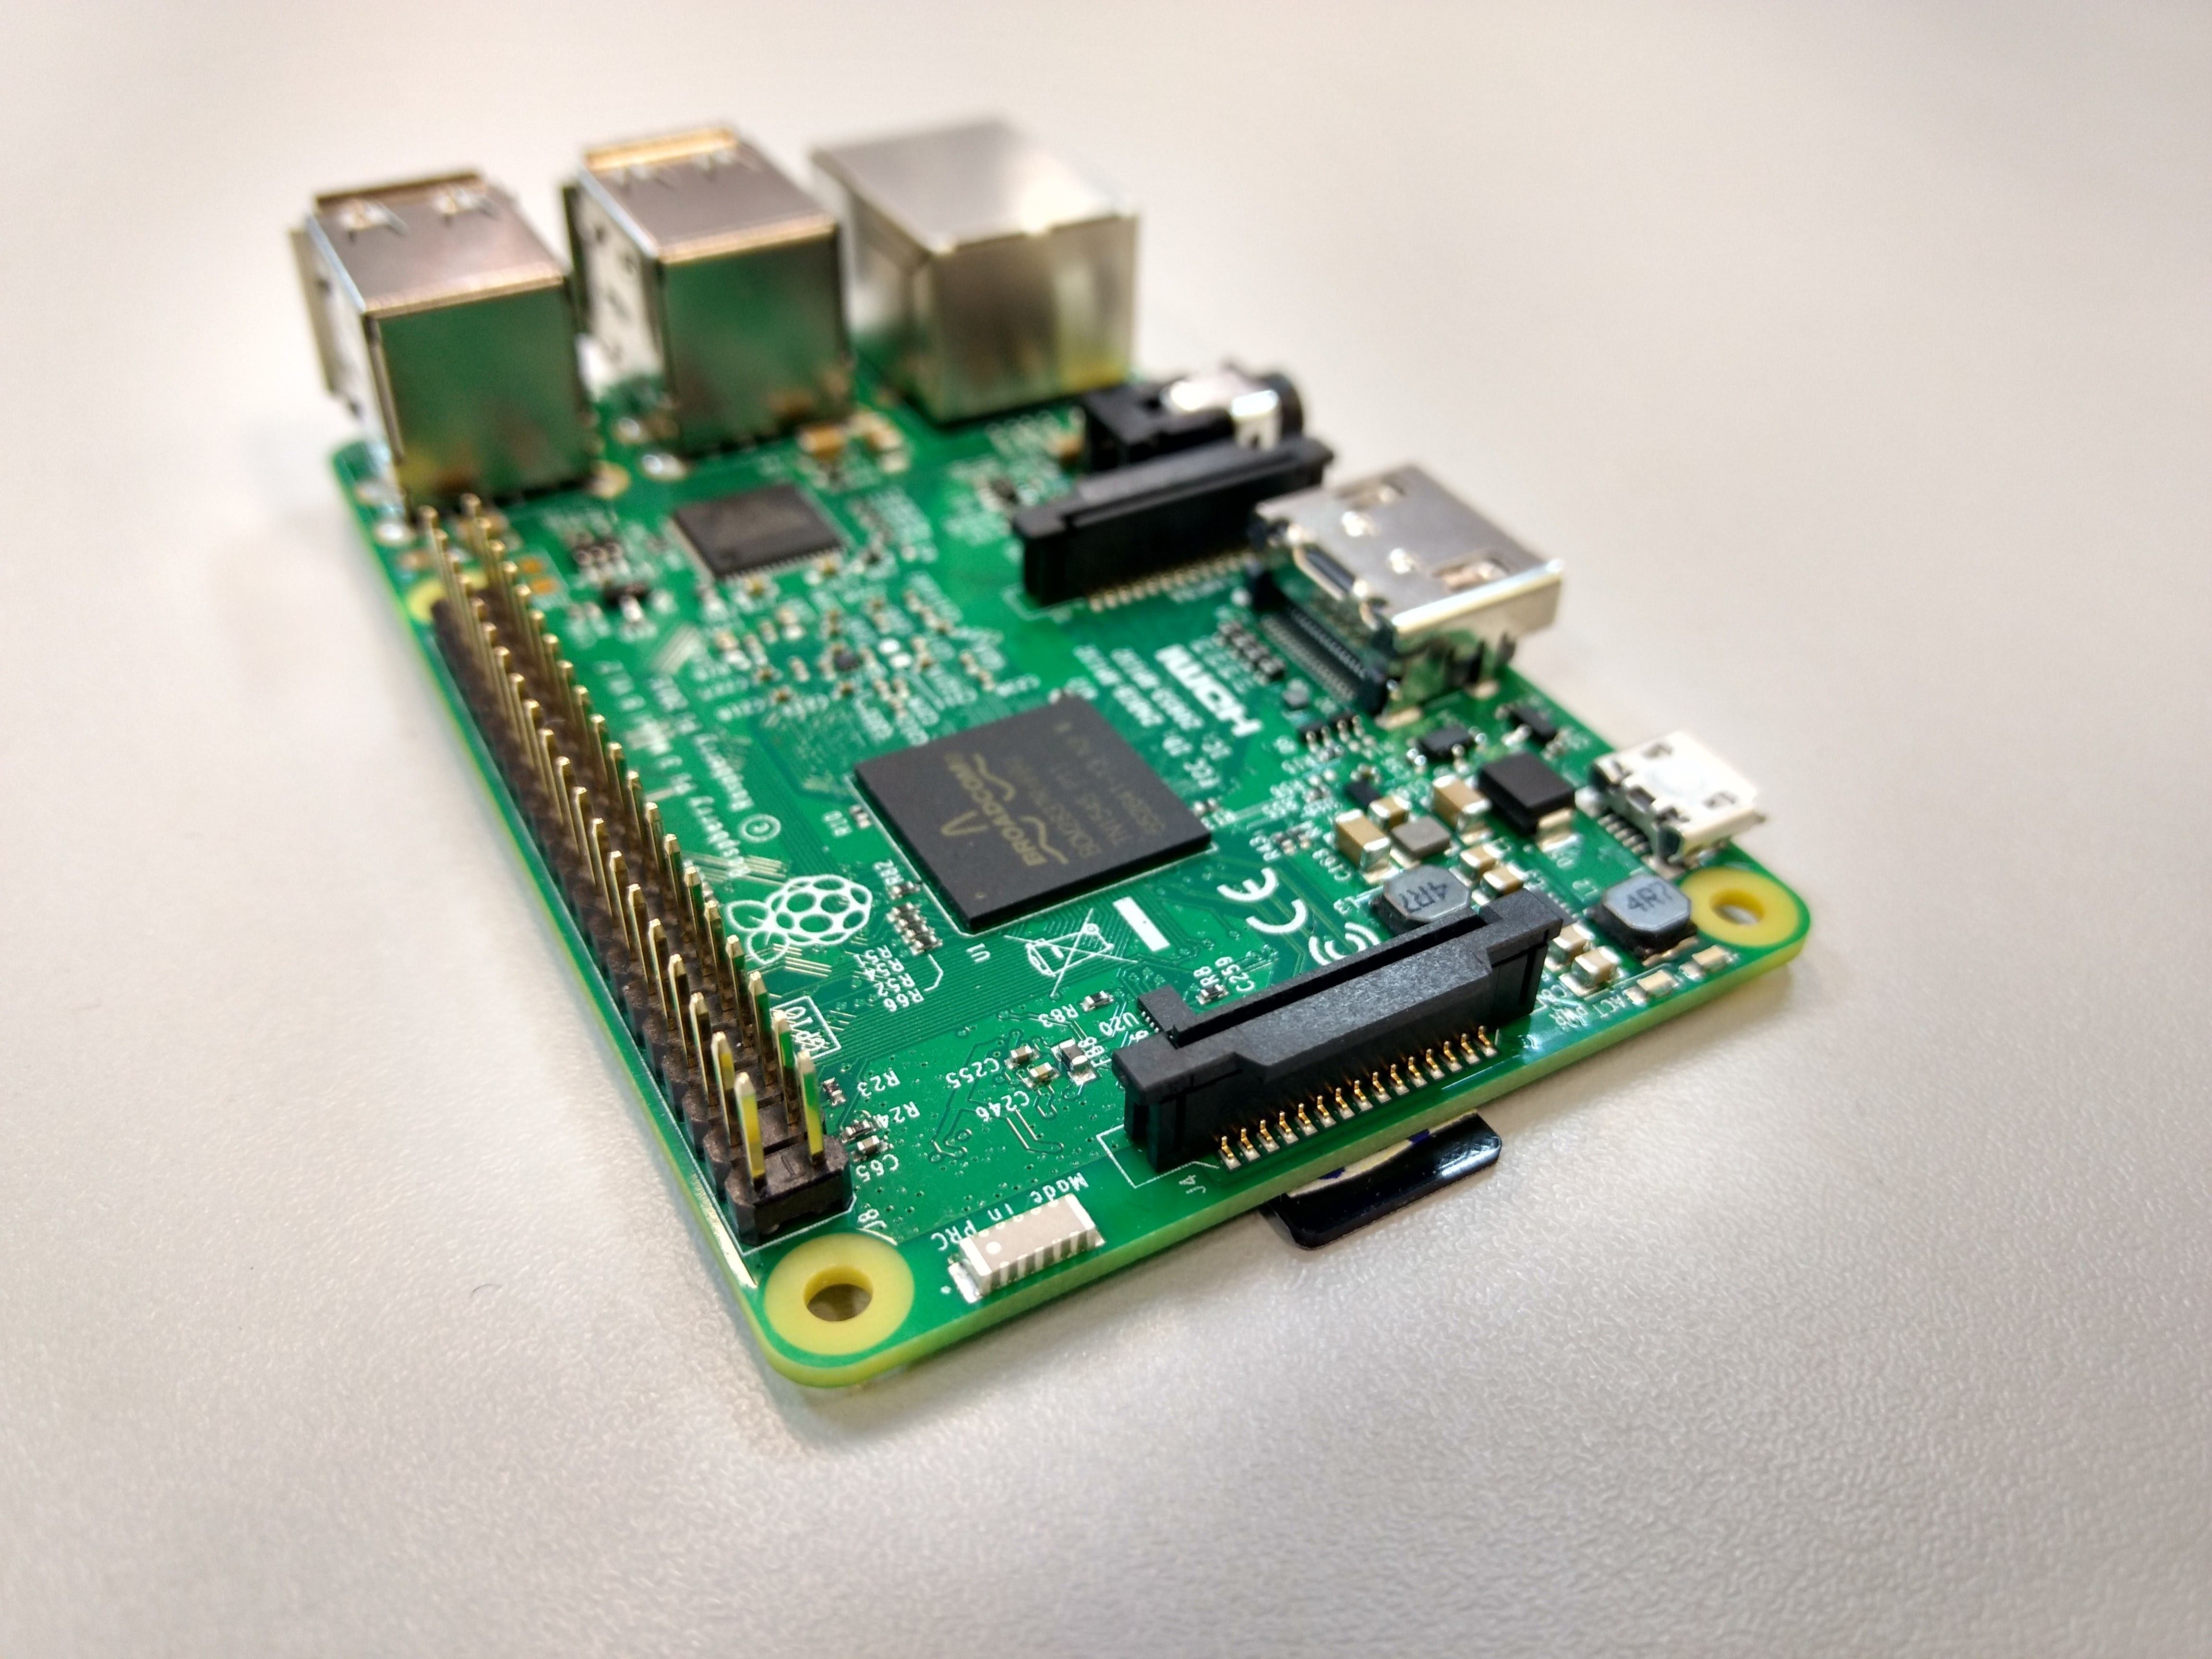
\includegraphics[width=1\textwidth]{040-plataformas/RPi-WiFi-dongles/rpi-onboard.jpg}
	\end{center}
	\legend{Fonte: Elaborada pelo autor}
\end{figure}


Sem modo promiscuo

\begin{figure}[htb]
	\caption{\label{fig:modulos-esp}Dongle WiFi Dlink}
	\begin{center}
		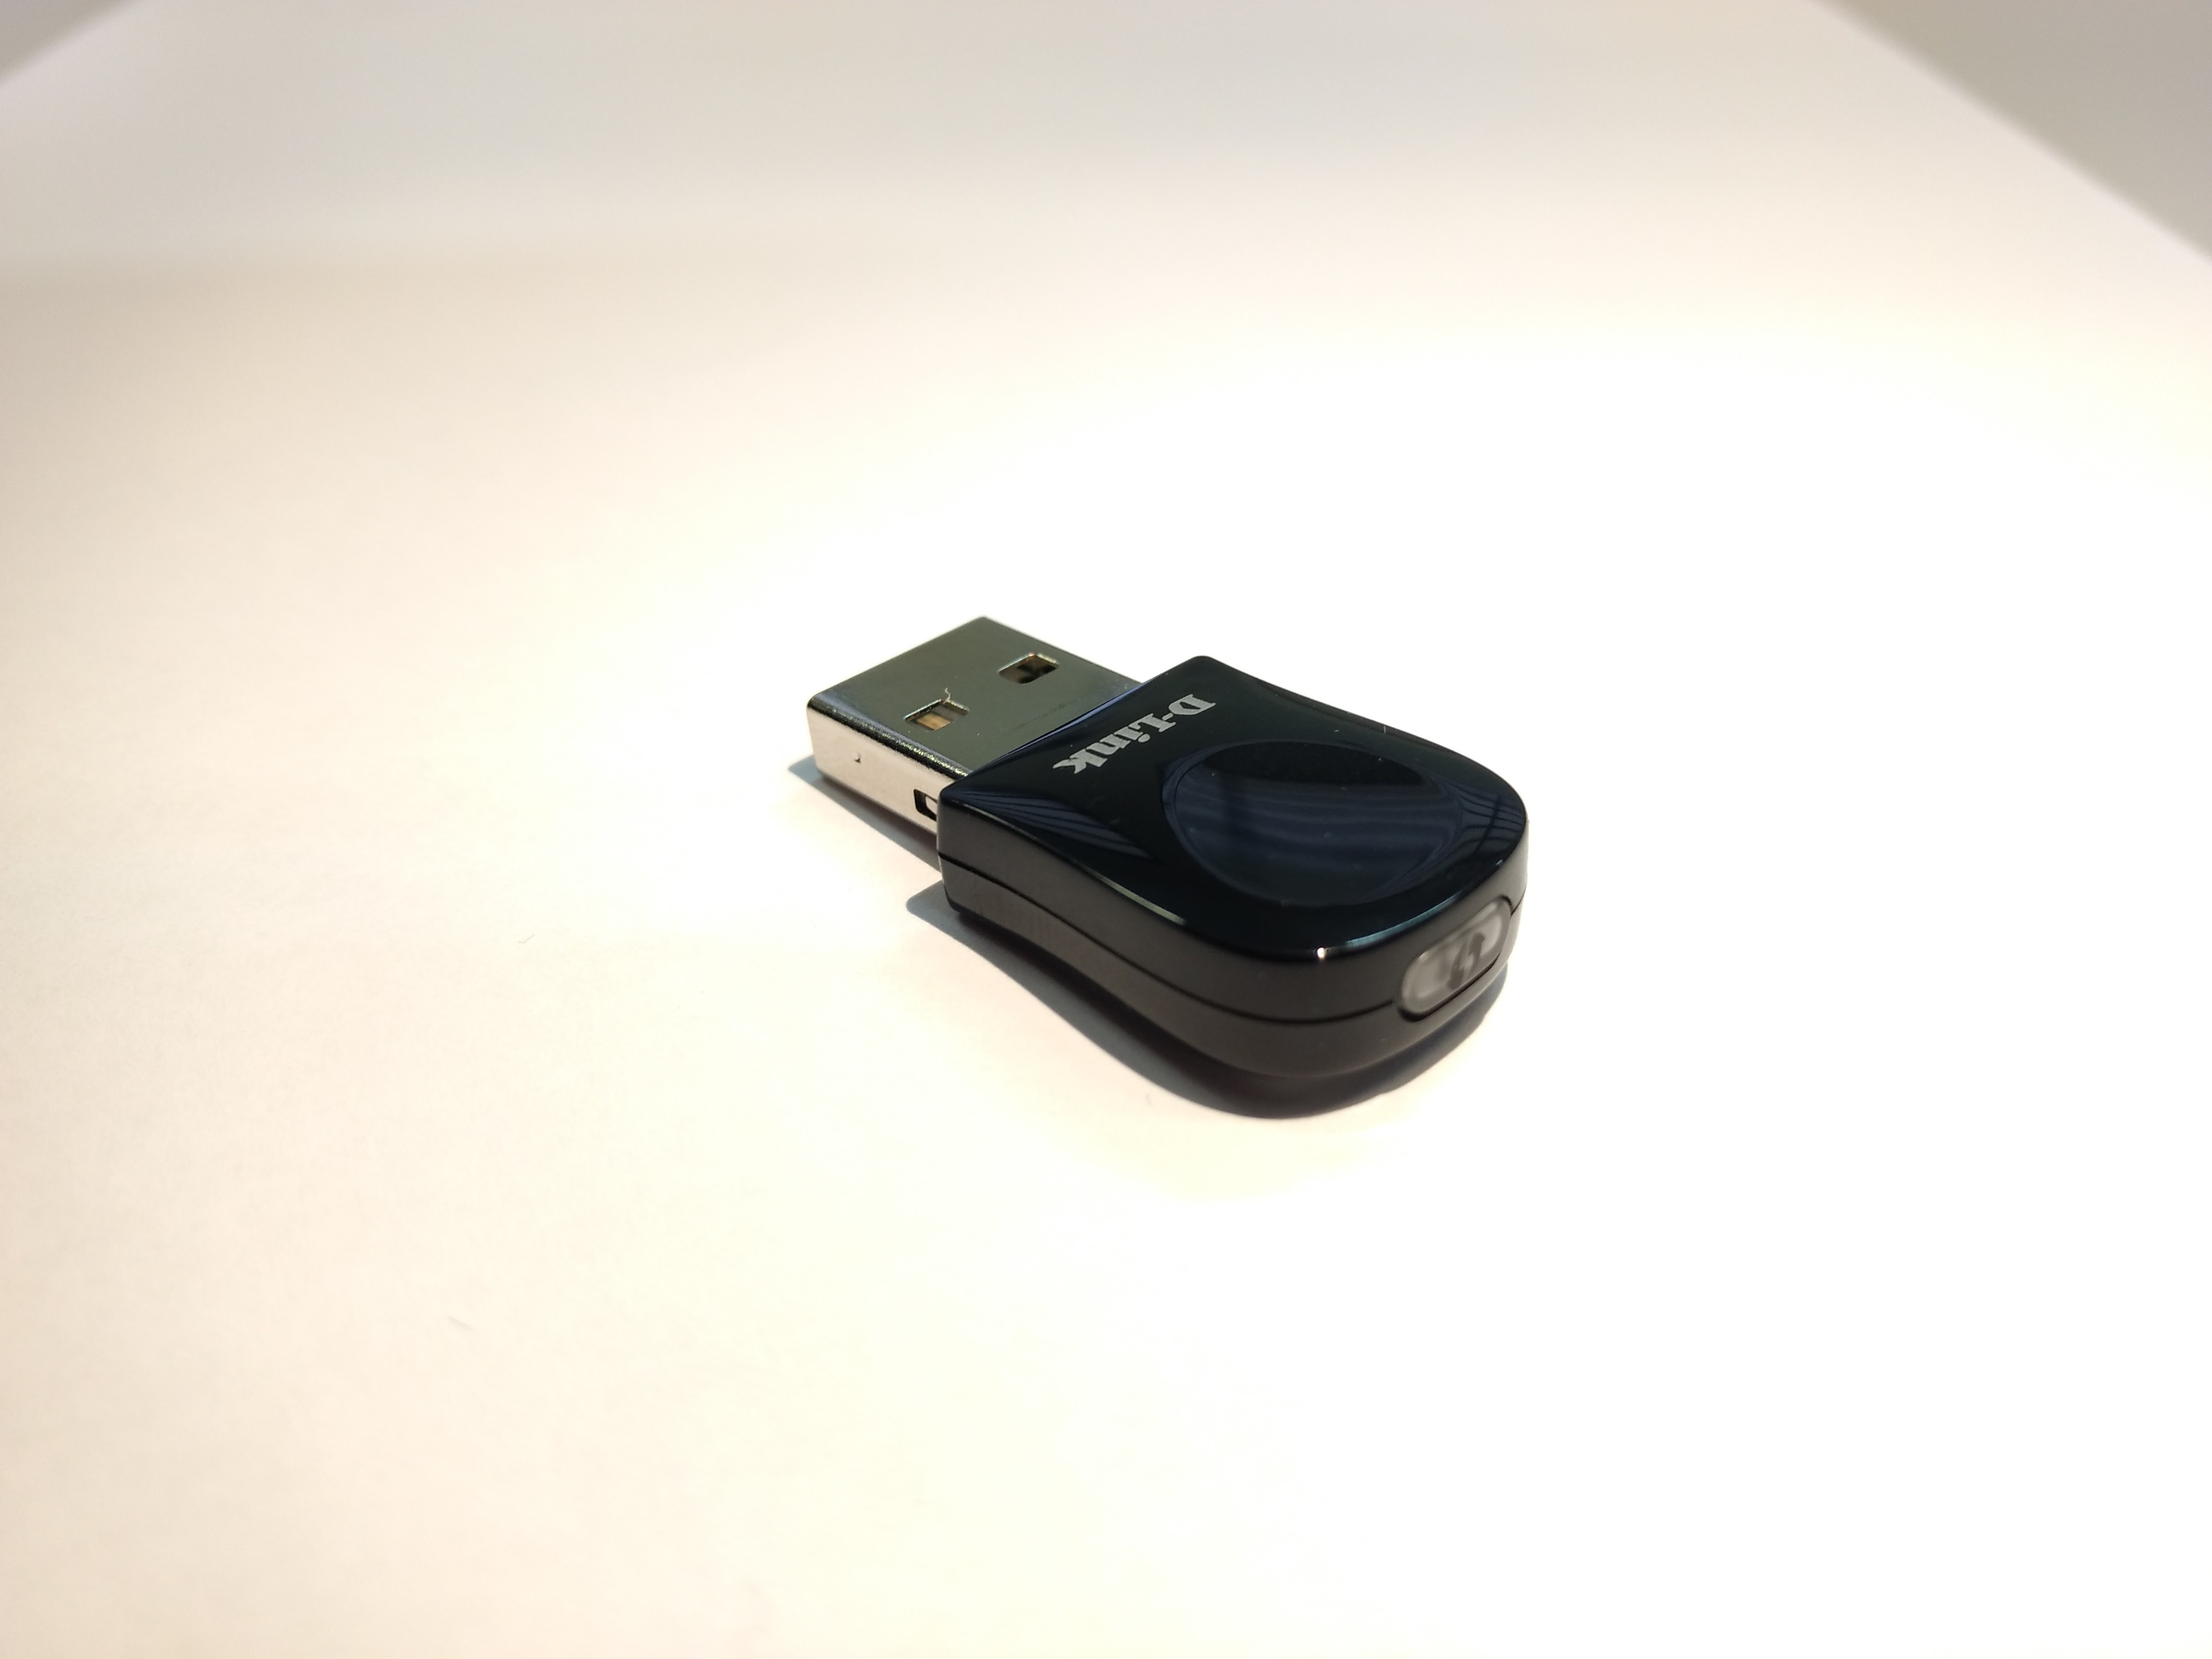
\includegraphics[width=1\textwidth]{040-plataformas/RPi-WiFi-dongles/dlink.jpg}
	\end{center}
	\legend{Fonte: Elaborada pelo autor}
\end{figure}


Com modo promiscuo

\begin{figure}[htb]
	\caption{\label{fig:modulos-esp}Dongle WiFi Ralink EPUB}
	\begin{center}
		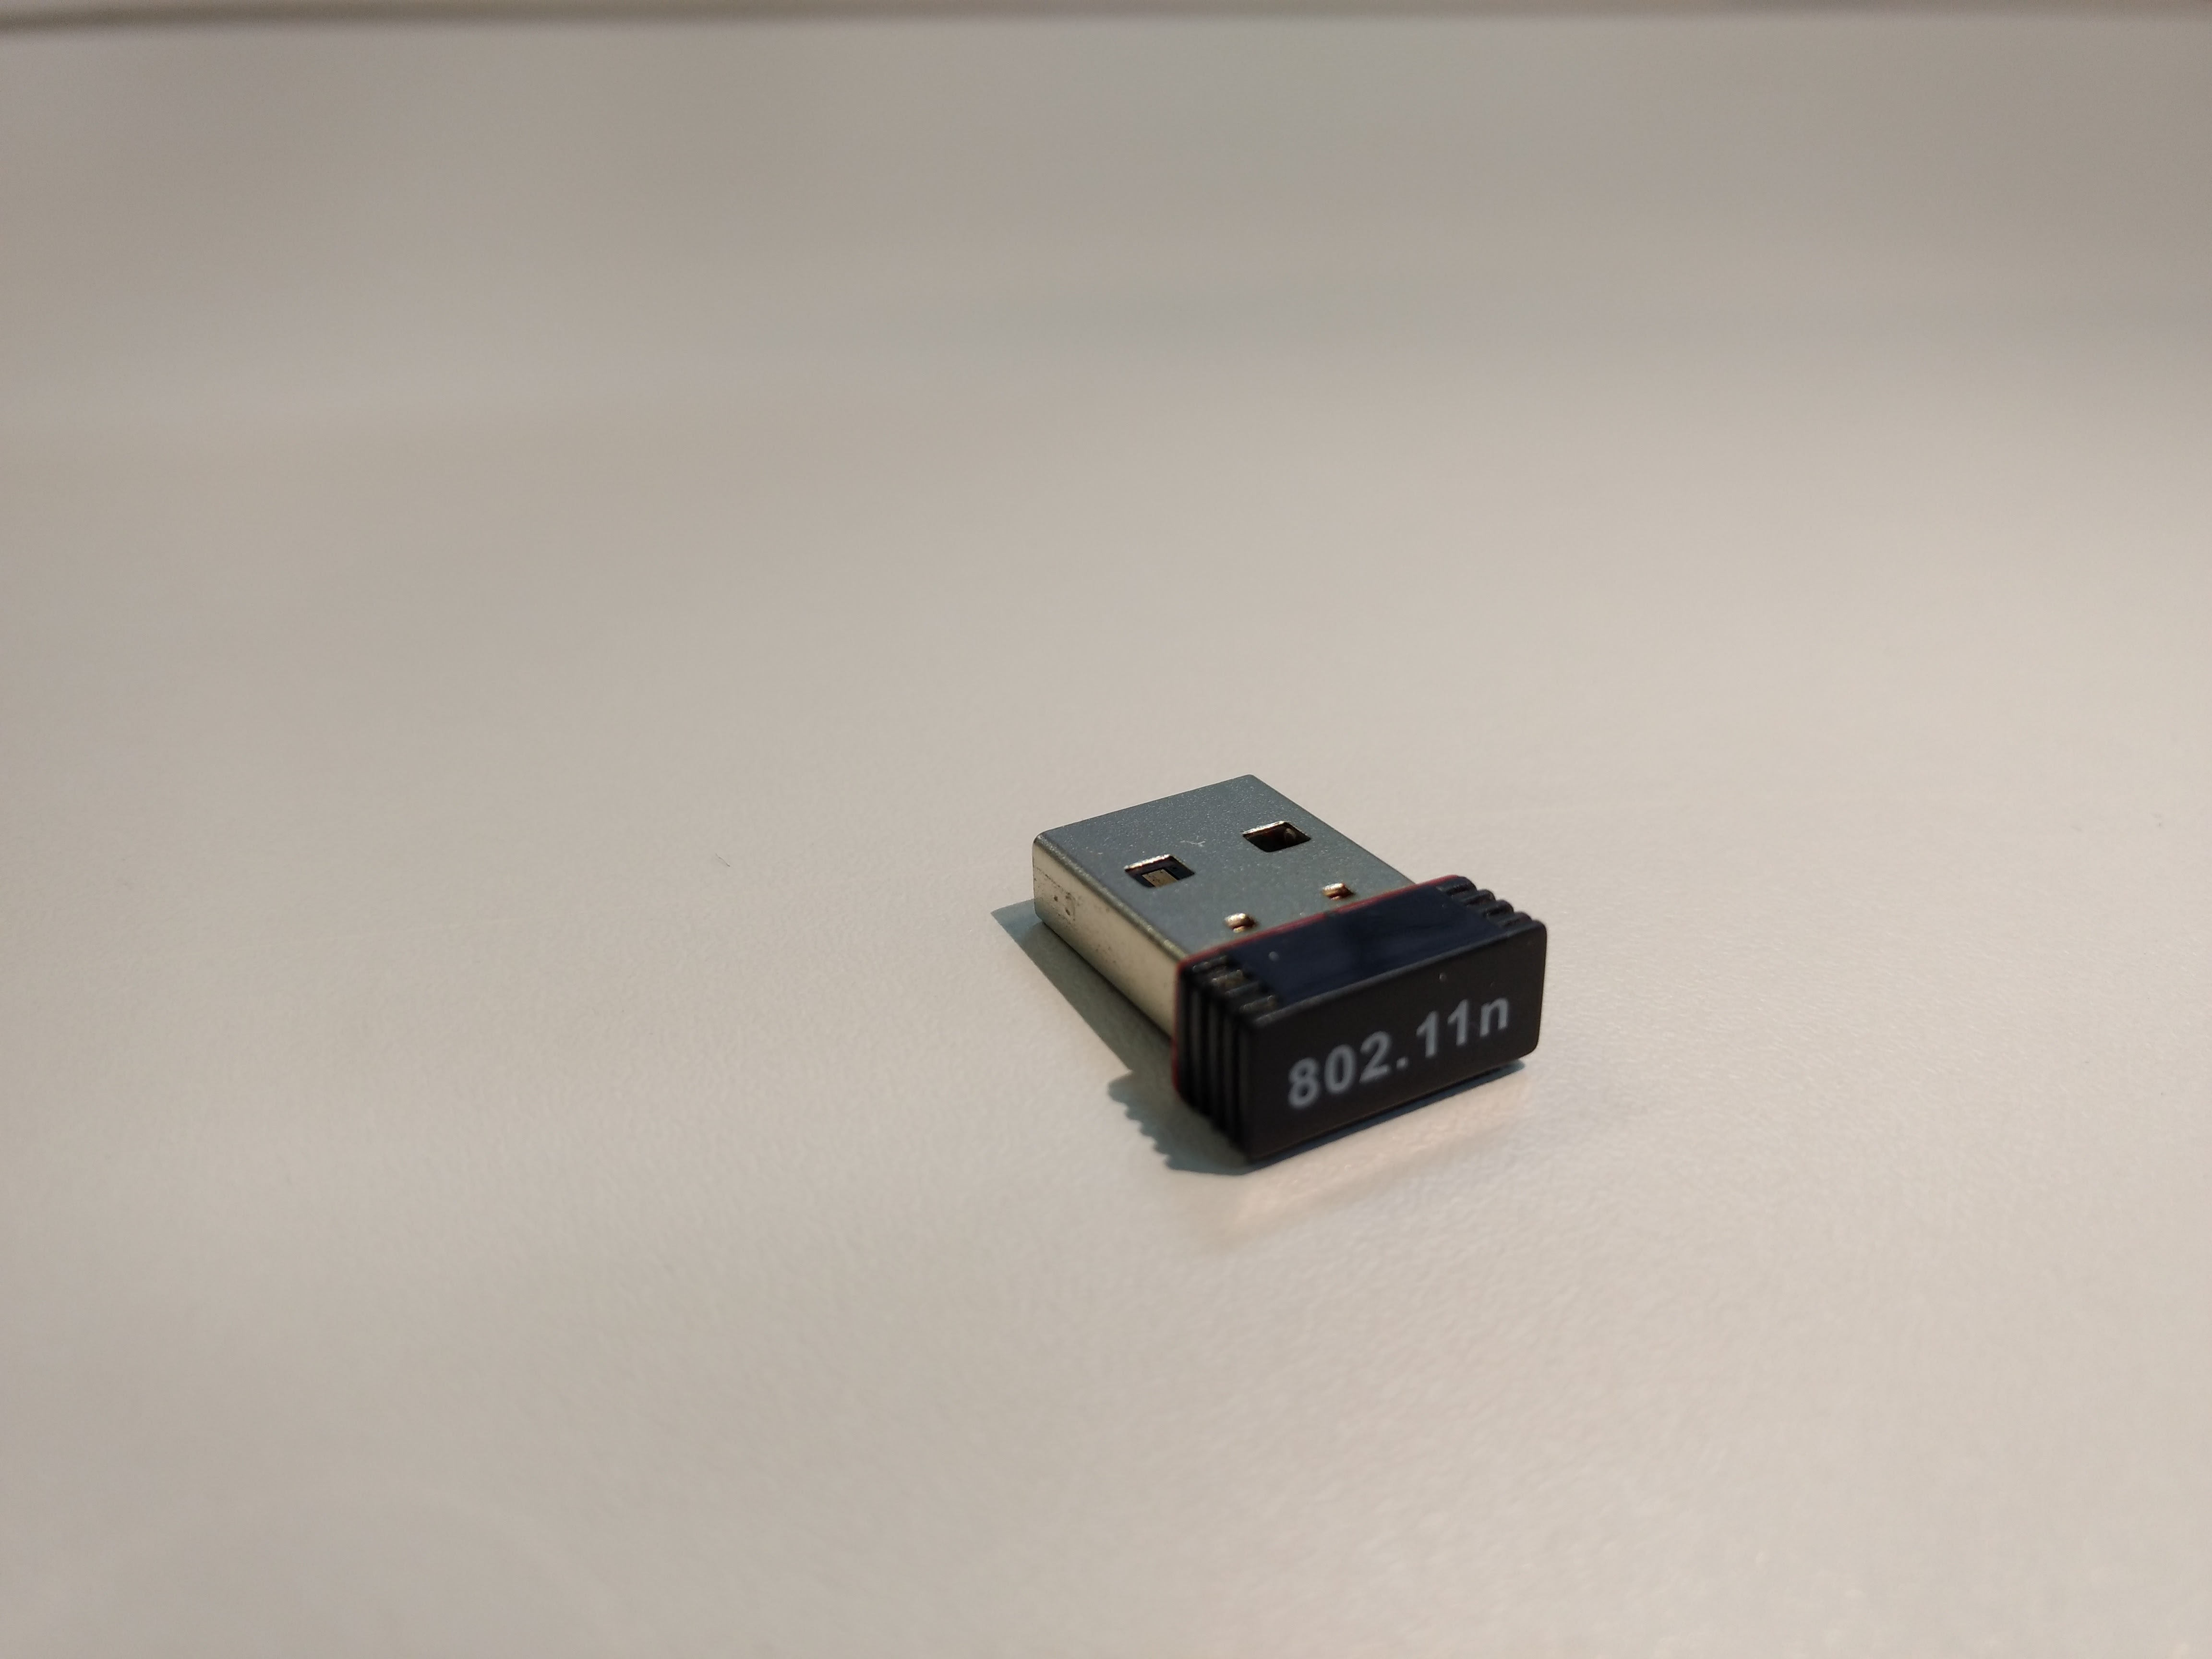
\includegraphics[width=1\textwidth]{040-plataformas/RPi-WiFi-dongles/ralink-epub.jpg}
	\end{center}
	\legend{Fonte: Elaborada pelo autor}
\end{figure}

Com modo promiscuo

\begin{figure}[htb]
	\caption{\label{fig:modulos-esp}Dongle WiFi Ralink}
	\begin{center}
		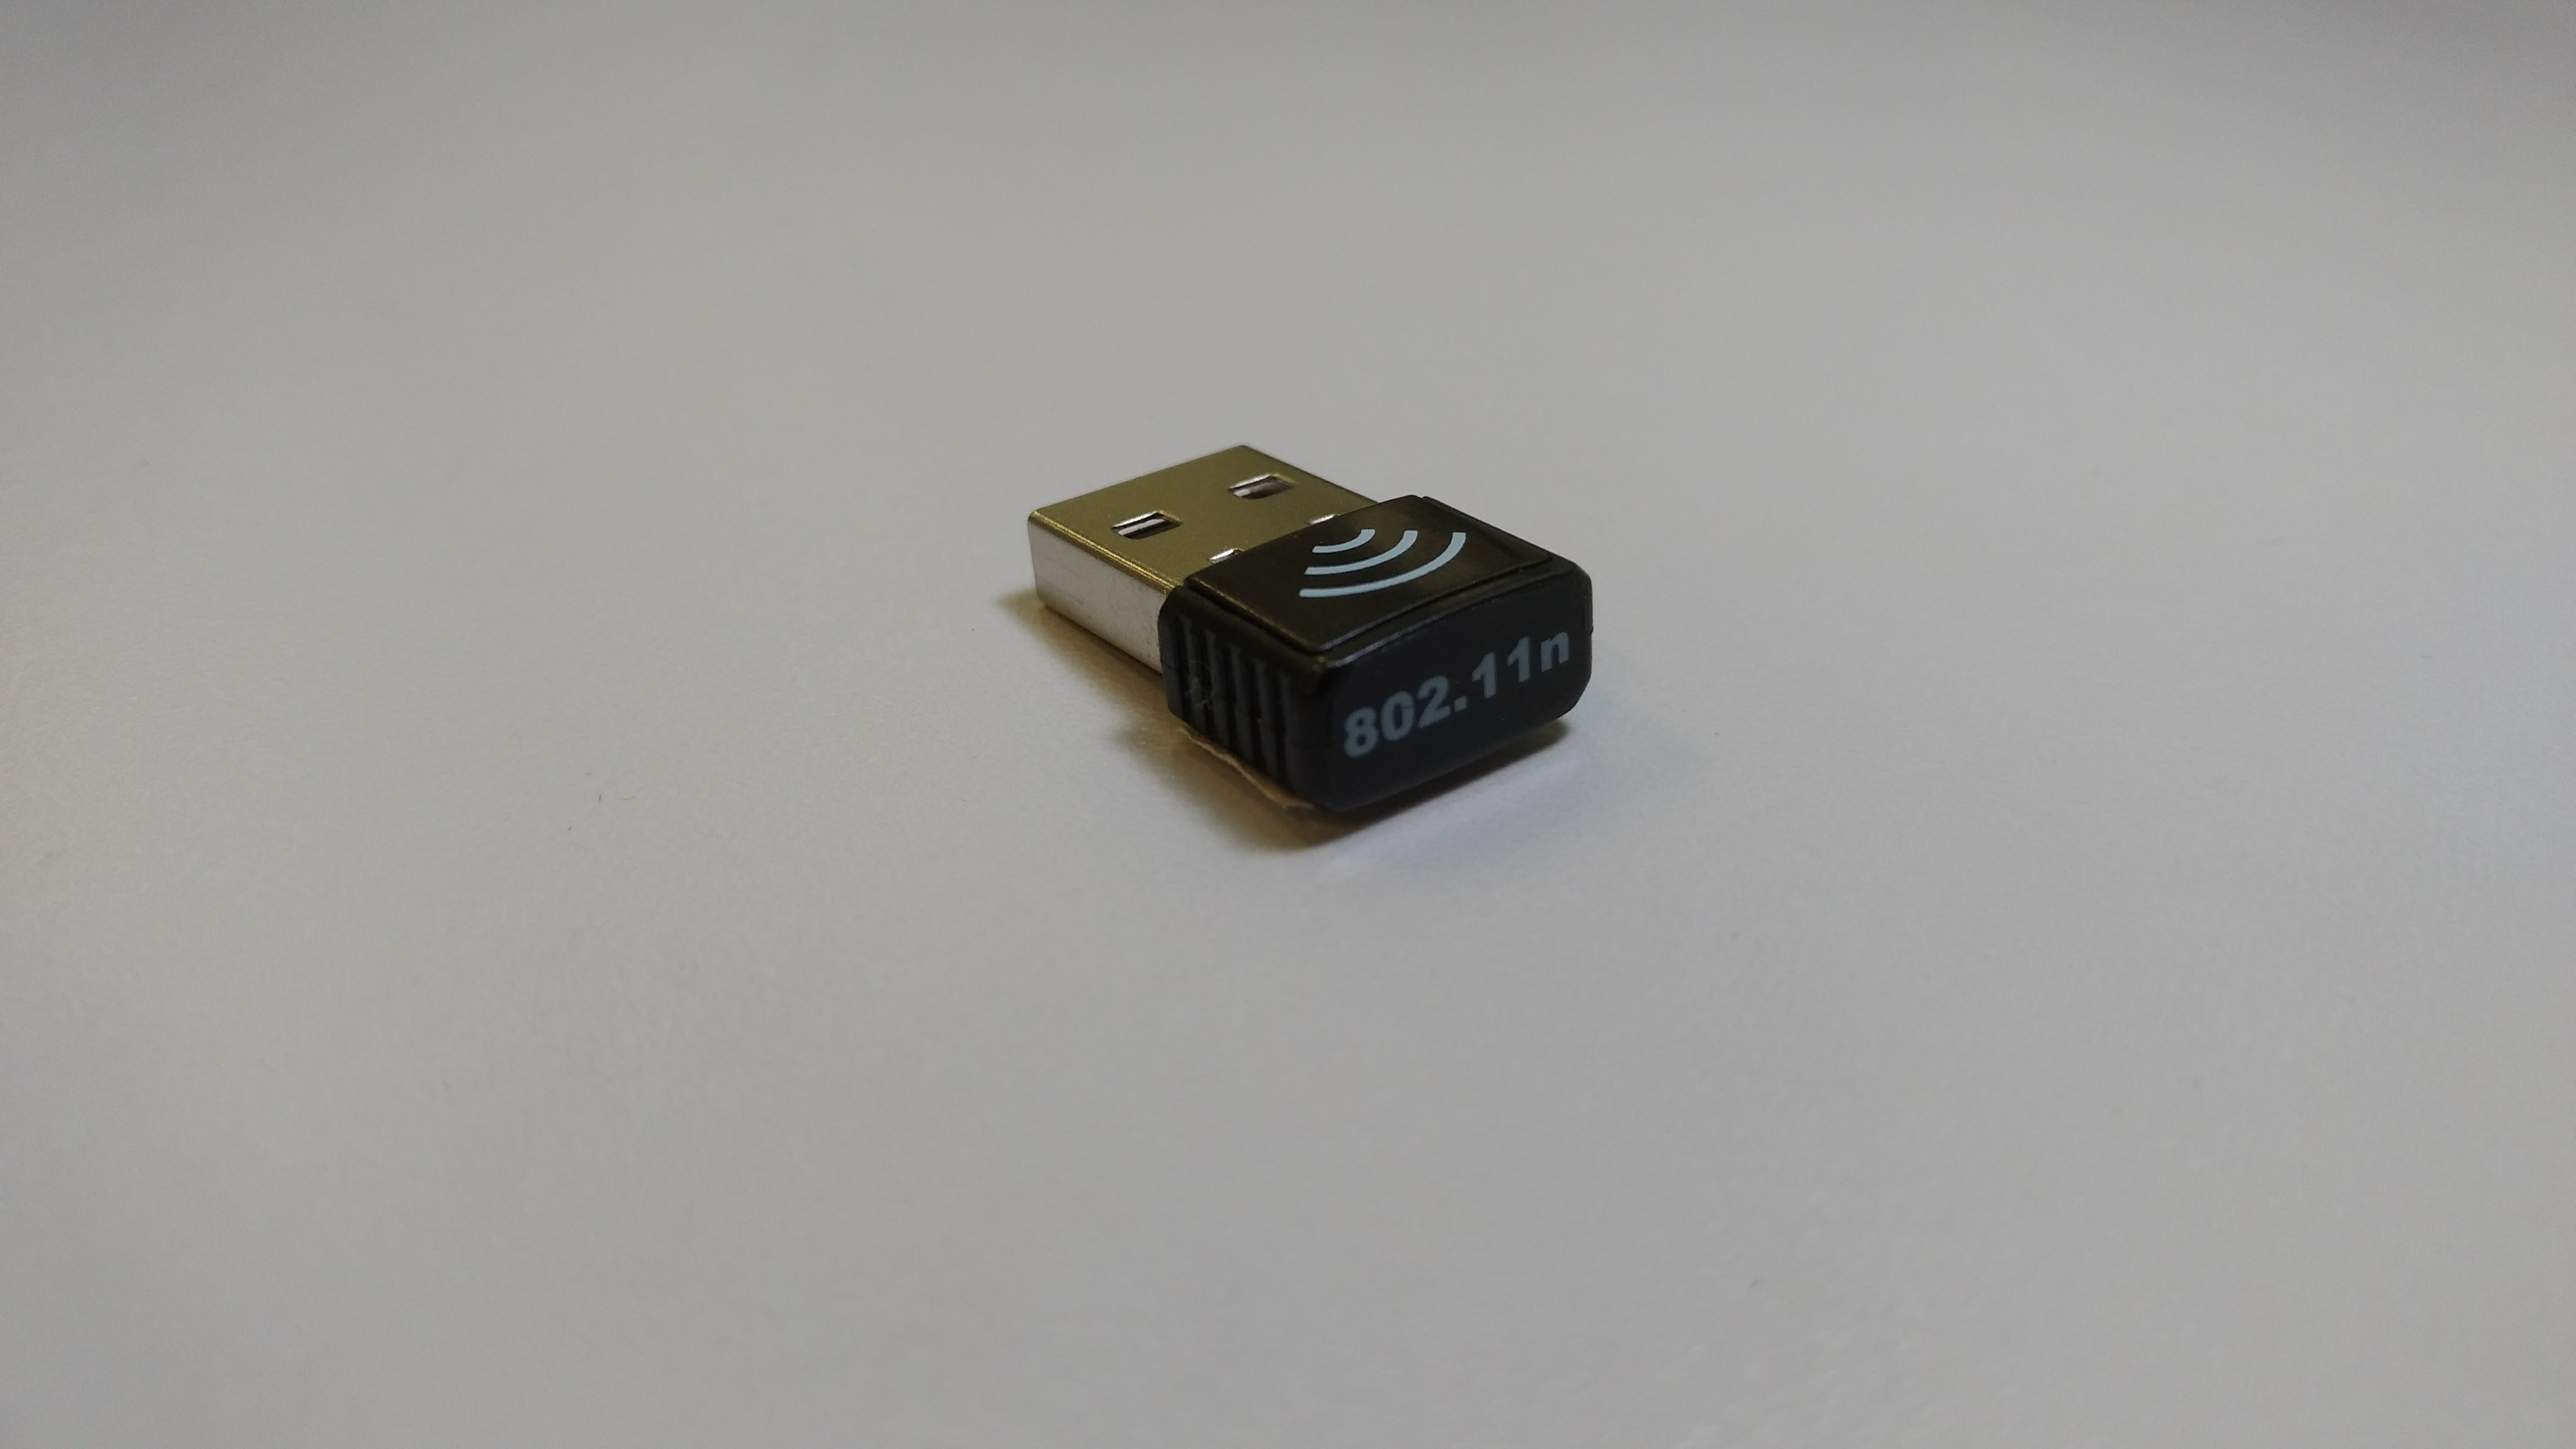
\includegraphics[width=1\textwidth]{040-plataformas/RPi-WiFi-dongles/ralink.jpg}
	\end{center}
	\legend{Fonte: Elaborada pelo autor}
\end{figure}
